% !TEX program = pdflatex
\documentclass[11pt,letterpaper]{article}

% --- Paquetes Esenciales
\usepackage[spanish,es-noshorthands]{babel}
\usepackage[utf8]{inputenc}
\usepackage[T1]{fontenc}
\usepackage{lmodern}
\usepackage{microtype}
\usepackage{geometry}
\geometry{margin=1in}
\usepackage{amsmath,amssymb,amsfonts,mathtools}
\usepackage{bm}

% --- Paquetes de Estilo y Formato
\usepackage{graphicx}
\usepackage{xcolor}
\usepackage{booktabs}
\usepackage{enumitem}
\usepackage{siunitx}
\usepackage{algorithm}
\usepackage{algorithmic}
\sisetup{locale=ES,per-mode=symbol,detect-weight=true,detect-inline-weight=math}
\usepackage[hidelinks]{hyperref} % Oculta los recuadros de color en los links
\hypersetup{colorlinks=true,linkcolor=blue,citecolor=teal,urlcolor=magenta}
\usepackage{caption}
\usepackage{subcaption}
\usepackage{tocloft}
\usepackage{physics}
\usepackage{cleveref}
\usepackage{float}

% --- Paquete para mejorar el diseño de las secciones
\usepackage{titlesec}
\titleformat{\section}{\normalfont\Large\bfseries}{\thesection}{1em}{}[\titlerule]

% --- Macros (Comandos personalizados)
\newcommand{\vx}{v_x}
\newcommand{\vy}{v_y}
\newcommand{\ux}{u}             % usaremos u := v_x en las fórmulas
\newcommand{\vyc}{v}            % y v := v_y
\newcommand{\Om}{\Omega}
\newcommand{\RR}{\mathbb{R}}
\newcommand{\dd}{\,\mathrm{d}}
\newcommand{\Rey}{\mathrm{Re}}
\newcommand{\Oh}{\mathcal{O}}
\newcommand{\Lap}{\nabla^2}
\DeclareMathOperator{\sgn}{sgn}

% --- Inicio del Documento
\begin{document}

% --- Portada Personalizada
\begin{titlepage}
    \centering
    
    % --- Logo ---
    \includegraphics[width=3cm]{univalle.jpg} 
    
    \vspace{1.5cm}
    
    {\huge\bfseries Universidad del Valle \par}
    
    \vspace{2cm}
    
    {\Large\scshape Simulación y Computación Numérica \par}
    
    \vspace{0.5cm}
    
    {\large Grupo 6 \par}
    
    \vspace{0.5cm}
    
    {\large Profesora: María Patricia Trujillo \par}
    
    \vfill
    
    {\Huge\bfseries Informe de Avance \par}
    \vspace{0.5cm}
    {\LARGE Simulación de Flujo Laminar Incompresible con Obstáculos \par}
    \vspace{0.25cm}
    {\Large\itshape Discretización de Navier--Stokes 2D, Mallas, Ecuaciones de Borde y Preparación del Método de Newton--Raphson \par}
    
    \vfill
    
    {\large\textbf{Presentado por:} \par}
    \vspace{0.5cm}
    {\large Juan David Rincón \par}
    {\large Maria Juliana Saavedra \par}
    {\large Libardo Alejandro Quintero \par}
    
    \vfill
    
    {\large \today \par}
    
\end{titlepage}


\begin{document}
\tableofcontents
\newpage

\section*{Resumen}
Se presenta el avance del proyecto de simulación de flujo incompresible en 2D alrededor de dos vigas sumergidas. Partimos del sistema de Navier--Stokes estacionario y la ecuación de continuidad, restringidos a flujo bidimensional en un canal rectangular. Se detalla la formulación continua, la discretización por diferencias finitas centradas en malla uniforme ($h_x=h_y=h=8$), y se derivan explícitamente las \textbf{nueve ecuaciones especiales} que surgen al imponer condiciones de contorno (cuatro lados y cuatro esquinas) más la condición de no deslizamiento en las vigas. Mostramos dos configuraciones de malla: la original ($N_x=400$, $N_y=40$) y una versión reducida para acelerar prototipado ($N'_x=50$, $N'_y=5$ puntos interiores). Finalmente, se describe la \emph{estrategia de inicialización} de velocidades para el método de Newton--Raphson y los \emph{criterios de parada} del solver.
\newpage

\section{Geometría, Mallas y Condiciones de Frontera}

\subsection{Configuraciones de Malla inicial supuesta}
\subsubsection{Dominio y Obstáculos}
El dominio computacional es un canal rectangular $\Om$ con dos vigas sólidas internas (A y B). Las condiciones de velocidad $\ux$ en las fronteras del canal son:
\begin{itemize}[leftmargin=1.25em]
    \item \textbf{Izquierda (Inlet \texttt{F})}: Perfil de entrada impuesto, $\ux=V_0$.
    \item \textbf{Superior (Pared \texttt{G})}: Condición de pared, $\ux=V0$.
    \item \textbf{Derecha (Outlet \texttt{H})}: Perfil de salida, $\ux=0$.
    \item \textbf{Inferior (Pared \texttt{EA})}: Condición de pared, $\ux=0$.
\end{itemize}
Sobre las superficies de las vigas A y B se impone la condición de no deslizamiento, es decir, $\ux=0$ y $\vyc=0$.


Se trabajan dos escalas de malla para facilitar el desarrollo:
\begin{enumerate}
    \item \textbf{Malla Original (Referencia):} Dimensiones $N_x=400$, $N_y=40$ con paso $h=1$. Las vigas se ubican en las coordenadas físicas:
    \[
    \text{Viga A: } x\in[176,232],\ y\in[1,16], \qquad
    \text{Viga B: } x\in[296,400],\ y\in[32,40].
    \]
    \begin{figure}[H]
    \centering
    \includegraphics[width=0.8\linewidth]{inicial.png}
    \caption{Esquema del dominio computacional inicial, mostrando la malla, la ubicación de las vigas A y B, y las condiciones de frontera.}
    \label{fig:placeholder}
    
\end{figure}
\end{enumerate}
\subsection{Malla Reducida con condiciones de frontera modificadas para el desarrollo (Actual):}

Para acelerar las pruebas, la malla se comprime por un factor $s=8$, resultando en $N'_x=50$ y $N'_y=5$ puntos interiores. Esta versión a escala ($h=8$) permite validar el código y los algoritmos de forma eficiente.

\textbf{Modificación de fronteras:} A diferencia de la malla original, en esta versión la frontera superior tiene $\ux=0$ (en lugar de $V_0$), simplificando el problema para la fase de desarrollo. El resto de condiciones de frontera y la condición de no deslizamiento en las vigas se mantienen igual.

\subsubsection{Ubicación de las Vigas en la Malla Reducida}
Con el factor de escalamiento $s=8$ y el espaciado de malla $h=8$, las vigas se ubican en las siguientes coordenadas físicas en la malla reducida actual:
\[
\text{Viga A (Inferior): } x\in[176,232],\ y\in[8,120], \qquad
\text{Viga B (Superior): } x\in[296,400],\ y\in[32,40].
\]

Estas coordenadas físicas corresponden a las siguientes posiciones en índices de malla (considerando que cada celda tiene tamaño $h=8$):
\begin{itemize}
    \item \textbf{Viga A (Inferior):} Columnas $j\in[22,29]$, Filas $i\in[1,2]$
    \item \textbf{Viga B (Superior):} Columnas $j\in[37,50]$, Filas $i\in[4,5]$
\end{itemize}

    \includegraphics[width=1\linewidth]{malla_2.png}

\newpage

\section{Discretización por Diferencias Finitas (DF): Paso a Paso}
El núcleo del método numérico consiste en transformar la ecuación diferencial parcial continua en un sistema de ecuaciones algebraicas que pueden ser resueltas en una computadora. Este proceso se realiza mediante la discretización del dominio y de las derivadas. A continuación, se detalla el procedimiento paso a paso.

\subsection{Paso 1: Ecuación de Partida Simplificada}
Partimos de la ecuación de momento en la dirección $x$ (NSx), que describe el balance de fuerzas en el fluido:
\[
\nu\left(\partial_{xx}\ux+\partial_{yy}\ux\right) = \ux\,\partial_x\ux + \vyc\,\partial_y\ux + \frac{1}{\rho}\,\partial_x P
\]
Aplicando las simplificaciones establecidas para esta fase del proyecto (viscosidad cinemática $\nu=1$ y gradiente de presión nulo $\partial_x P = 0$), la ecuación a discretizar se reduce a:
\begin{equation}
\partial_{xx}\ux+\partial_{yy}\ux = \ux\,\partial_x\ux + \vyc\,\partial_y\ux
\label{eq:cont-simplificada}
\end{equation}
Esta ecuación balancea los términos de difusión (izquierda) con los términos convectivos (derecha).

\subsection{Paso 2: Aproximación de las Derivadas}
El siguiente paso es reemplazar cada derivada parcial por su aproximación en diferencias finitas centradas en un nodo genérico $(i,j)$ de la malla. Estas aproximaciones tienen un error de segundo orden, $\mathcal{O}(h^2)$, lo que las hace adecuadas para obtener resultados precisos.

\begin{itemize}
    \item \textbf{Términos de difusión (segundas derivadas):}
    \begin{align*}
    \partial_{xx}\ux\big|_{i,j} &\approx \frac{\ux_{i+1,j}-2\ux_{i,j}+\ux_{i-1,j}}{h_x^2} \\
    \partial_{yy}\ux\big|_{i,j} &\approx \frac{\ux_{i,j+1}-2\ux_{i,j}+\ux_{i,j-1}}{h_y^2}
    \end{align*}
    
    \item \textbf{Términos convectivos (primeras derivadas):}
    \begin{align*}
    \partial_x \ux\big|_{i,j} &\approx \frac{\ux_{i+1,j}-\ux_{i-1,j}}{2h_x} \\
    \partial_y \ux\big|_{i,j} &\approx \frac{\ux_{i,j+1}-\ux_{i,j-1}}{2h_y}
    \end{align*}
\end{itemize}
\subsection{Paso 3: Sustitución en la Ecuación Continua}
Ahora, sustituimos estas expresiones discretas en la ecuación continua simplificada (\cref{eq:cont-simplificada}):
\[
\frac{\ux_{i+1,j}-2\ux_{i,j}+\ux_{i-1,j}}{h_x^2} + \frac{\ux_{i,j+1}-2\ux_{i,j}+\ux_{i,j-1}}{h_y^2} = \ux_{i,j}\left(\frac{\ux_{i+1,j}-\ux_{i-1,j}}{2h_x}\right) + \vyc_{i,j}\left(\frac{\ux_{i,j+1}-\ux_{i,j-1}}{2h_y}\right)
\]
Esta ecuación es la representación algebraica completamente discreta de nuestra ecuación diferencial.

\subsection{Paso 4: Aplicación de Parámetros de la Malla}
Para este proyecto, en la malla de desarrollo actual, se establece que el espaciado es uniforme con $\boldsymbol{h_x = h_y = h = 8}$. Al multiplicar toda la ecuación por $h^2$, el coeficiente de los términos convectivos se convierte en:
\[
\text{Coeficiente} = \frac{h^2}{2h} = \frac{h}{2} = \frac{8}{2} = 4
\]
La ecuación balanceada queda:
\begin{equation}
(\ux_{i+1,j}-2\ux_{i,j}+\ux_{i-1,j}) + (\ux_{i,j+1}-2\ux_{i,j}+\ux_{i,j-1}) = 4\ux_{i,j}(\ux_{i+1,j}-\ux_{i-1,j}) + 4\vyc_{i,j}(\ux_{i,j+1}-\ux_{i,j-1})
\label{eq:disc-general}
\end{equation}
Agrupando los términos $\ux_{i,j}$ del lado izquierdo, obtenemos el factor $-4\ux_{i,j}$.

\subsection{Paso 5: Despeje de la Incógnita $\ux_{i,j}$}
El objetivo final es obtener una expresión explícita para $\ux_{i,j}$. Reorganizamos para despejar el término central $4\ux_{i,j}$, moviendo la suma de vecinos y restando los términos convectivos:
\[
4\ux_{i,j} = (\ux_{i+1,j}+\ux_{i-1,j}+\ux_{i,j+1}+\ux_{i,j-1}) - 4\ux_{i,j}(\ux_{i+1,j}-\ux_{i-1,j}) - 4\vyc_{i,j}(\ux_{i,j+1}-\ux_{i,j-1})
\]
Finalmente, dividimos por 4 para obtener la fórmula de iteración. 
\begin{equation}
\boxed{\;
\ux_{i,j}=\frac{1}{4}\Big[
\left(\ux_{i+1,j}+\ux_{i-1,j}+\ux_{i,j+1}+\ux_{i,j-1}\right)
- 4\,\ux_{i,j}\,(\ux_{i+1,j}-\ux_{i-1,j})
- 4\,\vyc_{i,j}\,(\ux_{i,j+1}-\ux_{i,j-1})
\Big]. \;} 
\label{eq:formula-centro}
\end{equation}
Esta ecuación es la piedra angular del modelo numérico para la malla escalada.

\newpage
\section{Las 9 Ecuaciones Especiales: Centro, Lados y Esquinas}
La fórmula \cref{eq:formula-centro} se adapta para los bordes sustituyendo los vecinos "fantasma" por las condiciones de frontera conocidas (ver Figura de la malla en la sección anterior).

\subsubsection{Caso 1: Nodo Central (Interior Puro)}
Se utiliza la Ecuación \ref{eq:formula-centro}:
\[
\ux_{i,j}=\frac{1}{4}\Big[ (\ux_{i+1,j}+\ux_{i-1,j}+\ux_{i,j+1}+\ux_{i,j-1})
- 4\ux_{i,j}(\ux_{i+1,j}-\ux_{i-1,j})
- 4\vyc_{i,j}(\ux_{i,j+1}-\ux_{i,j-1}) \Big]
\]

\subsubsection{Caso 2: Lado Izquierdo (Inlet F)}
Vecino izquierdo $\ux_{i-1,j} = V_0$.
\[
\ux_{1,j}=\frac{1}{4}\Big[ (\ux_{2,j}+V_0+\ux_{1,j+1}+\ux_{1,j-1})
- 4\ux_{1,j}(\ux_{2,j}-V_0)
- 4\vyc_{1,j}(\ux_{1,j+1}-\ux_{1,j-1}) \Big]
\]

\subsubsection{Caso 3: Lado Derecho (Outlet H)}
Vecino derecho $\ux_{i+1,j} = 0$.
\[
\ux_{N_x,j}=\frac{1}{4}\Big[ (0+\ux_{N_x-1,j}+\ux_{N_x,j+1}+\ux_{N_x,j-1})
- 4\ux_{N_x,j}(0-\ux_{N_x-1,j})
- 4\vyc_{N_x,j}(\ux_{N_x,j+1}-\ux_{N_x,j-1}) \Big]
\]

\subsubsection{Caso 4: Lado Superior (Pared G)}
Vecino superior $\ux_{i,j+1} = V_0$.
\[
\ux_{i,N_y}=\frac{1}{4}\Big[ (\ux_{i+1,N_y}+\ux_{i-1,N_y}+V_0+\ux_{i,N_y-1})
- 4\ux_{i,N_y}(\ux_{i+1,N_y}-\ux_{i-1,N_y})
- 4\vyc_{i,N_y}(V_0-\ux_{i,N_y-1}) \Big]
\]

\subsubsection{Caso 5: Lado Inferior (Pared EA)}
Vecino inferior $\ux_{i,j-1} = 0$.
\[
\ux_{i,1}=\frac{1}{4}\Big[ (\ux_{i+1,1}+\ux_{i-1,1}+\ux_{i,2}+0)
- 4\ux_{i,1}(\ux_{i+1,1}-\ux_{i-1,1})
- 4\vyc_{i,1}(\ux_{i,2}-0) \Big]
\]

\subsubsection{Caso 6: Esquina Superior Izquierda (G$\cap$F)}
$U_L=V_0, U_T=V_0$.
\[
\ux_{1,N_y}=\frac{1}{4}\Big[ (\ux_{2,N_y}+V_0+V_0+\ux_{1,N_y-1})
- 4\ux_{1,N_y}(\ux_{2,N_y}-V_0)
- 4\vyc_{1,N_y}(V_0-\ux_{1,N_y-1}) \Big]
\]

\subsubsection{Caso 7: Esquina Superior Derecha (G$\cap$H)}
$U_R=0, U_T=V_0$.
\[
\ux_{N_x,N_y}=\frac{1}{4}\Big[ (0+\ux_{N_x-1,N_y}+V_0+\ux_{N_x,N_y-1})
- 4\ux_{N_x,N_y}(0-\ux_{N_x-1,N_y})
- 4\vyc_{N_x,N_y}(V_0-\ux_{N_x,N_y-1}) \Big]
\]

\subsubsection{Caso 8: Esquina Inferior Derecha (EA$\cap$H)}
$U_R=0, U_B=0$.
\[
\ux_{N_x,1}=\frac{1}{4}\Big[ (0+\ux_{N_x-1,1}+\ux_{N_x,2}+0)
- 4\ux_{N_x,1}(0-\ux_{N_x-1,1})
- 4\vyc_{N_x,1}(\ux_{N_x,2}-0) \Big]
\]

\subsubsection{Caso 9: Esquina Inferior Izquierda (EA$\cap$F)}
$U_L=V_0, U_B=0$.
\[
\ux_{1,1}=\frac{1}{4}\Big[ (\ux_{2,1}+V_0+\ux_{1,2}+0)
- 4\ux_{1,1}(\ux_{2,1}-V_0)
- 4\vyc_{1,1}(\ux_{1,2}-0) \Big]
\]

\paragraph{Nodos dentro de vigas (no--slip):} Para cualquier nodo $(i,j)$ que se encuentre dentro de las vigas A o B, se impone directamente $\ux_{i,j}=0$ y $\vyc_{i,j}=0$.
\section{Método de Solución: Newton--Raphson}

El conjunto de ecuaciones discretas forma un sistema algebraico no lineal de gran tamaño. Para resolverlo, se utiliza el método de Newton--Raphson, que busca la raíz del vector de residuales $\mathbf{F}(\mathbf{U})=0$. Cada iteración consiste en:

\[
J(\mathbf{U}^{(k)})\,\Delta \mathbf{U}^{(k)}=-\mathbf{F}(\mathbf{U}^{(k)}),\qquad
\mathbf{U}^{(k+1)}=\mathbf{U}^{(k)}+\Delta \mathbf{U}^{(k)}.
\]

Alternativamente, el método puede expresarse como:
\[
\mathbf{U}^{(k+1)} = \mathbf{U}^{(k)} - J^{-1}(\mathbf{U}^{(k)}) \cdot \mathbf{F}(\mathbf{U}^{(k)})
\]

\subsection{Geometría y Discretización del Dominio}

La geometría del problema (canal con dos bloques sólidos) se mostró en la sección de mallas.

Para la simulación, se utiliza una malla con las siguientes características:
\begin{itemize}
    \item Dimensiones del dominio: $L_x = 400$ unidades, $L_y = 40$ unidades
    \item Espaciamiento de malla: $h_x = h_y = h = 8$ unidades
    \item Número de nodos internos: $N_x = 50$ nodos en dirección $x$, $N_y = 5$ nodos en dirección $y$
    \item Total de nodos: $(N_x + 2) \times (N_y + 2) = 52 \times 7 = 364$ nodos
\end{itemize}

\subsection{Tabla de Parámetros de Simulación}

Para referencia rápida, la Tabla~\ref{tab:parametros} resume todos los parámetros numéricos y físicos utilizados en la simulación actual.

\begin{table}[H]
\centering
\begin{tabular}{|l|c|c|}
\hline
\textbf{Parámetro} & \textbf{Símbolo} & \textbf{Valor} \\
\hline
\multicolumn{3}{|c|}{\textbf{Parámetros Geométricos}} \\
\hline
Longitud del dominio & $L_x$ & 400 \\
Altura del dominio & $L_y$ & 40 \\
Espaciado de malla & $h$ & 8 \\
Nodos en dirección $x$ & $N_x$ & 50 \\
Nodos en dirección $y$ & $N_y$ & 5 \\
Total de nodos & $N_{\text{total}}$ & 364 \\
\hline
\multicolumn{3}{|c|}{\textbf{Parámetros Físicos}} \\
\hline
Velocidad de entrada & $V_0$ & 1 \\
Velocidad vertical & $V_y$ & $-0.000005$ \\
Viscosidad cinemática & $\nu$ & 1 \\
Densidad & $\rho$ & constante \\
\hline
\multicolumn{3}{|c|}{\textbf{Parámetros Numéricos}} \\
\hline
Tolerancia residual & $\varepsilon_F$ & $10^{-10}$ \\
Tolerancia cambio & $\delta_{\text{step}}$ & $10^{-8}$ \\
Iteraciones máximas Newton & $k_{\max}$ & 200 \\
Tolerancia gradiente conjugado & $\text{tol}_{\text{CG}}$ & $10^{-10}$ \\
Factor refinamiento visual & $f$ & 10 \\
\hline
\end{tabular}
\caption{Parámetros numéricos y físicos utilizados en la simulación con malla reducida.}
\label{tab:parametros}
\end{table}

La malla se estructura como una matriz de velocidades:
\[
\mathbf{U} = \begin{bmatrix}
v_{0,0} & v_{0,1} & v_{0,2} & \cdots & v_{0,50} & v_{0,51} \\
v_{1,0} & v_{1,1} & v_{1,2} & \cdots & v_{1,50} & v_{1,51} \\
v_{2,0} & v_{2,1} & v_{2,2} & \cdots & v_{2,50} & v_{2,51} \\
\vdots & \vdots & \vdots & \ddots & \vdots & \vdots \\
v_{6,0} & v_{6,1} & v_{6,2} & \cdots & v_{6,50} & v_{6,51}
\end{bmatrix}
\]

\subsection{Conversión Matriz-Vector}

Para aplicar el método de Newton-Raphson, la matriz de velocidades se convierte en un vector unidimensional. La transformación se realiza mediante:
\[
\text{índice vectorial} = i \times N_{\text{cols}} + j
\]
donde $i$ es el índice de fila, $j$ es el índice de columna, y $N_{\text{cols}} = 52$.

De forma inversa:
\[
\text{fila} = \left\lfloor \frac{\text{índice}}{52} \right\rfloor, \quad
\text{columna} = \text{índice} \bmod 52
\]

El vector resultante tiene dimensión $N_{\text{total}} = 364$ ecuaciones.

\subsection{Inicialización Informada de $\mathbf{U}^{(0)}$}

Una buena estimación inicial es clave para la convergencia del método de Newton-Raphson. Se diseña una estrategia que refleja la física esperada del flujo (disminución de velocidad de izquierda a derecha y de arriba a abajo).

\subsubsection{Generación de Intervalos Decrecientes}

La malla se divide en secciones tanto horizontal como verticalmente. Para la malla reducida ($50\times5$):

\paragraph{División Horizontal (Eje X):} 
Se define $d_h = 10$ divisiones horizontales. El paso entre valores es:
\[
\Delta_h = \frac{1}{2 \times d_h} = \frac{1}{20} = 0.05
\]

Esto genera una lista de valores decrecientes:
\[
L_h = [0.95, 0.90, 0.85, 0.80, 0.75, 0.70, 0.65, 0.60, 0.55, 0.50, 0.45, 0.40, 0.35, 0.30, 0.25, 0.20, 0.15, 0.10, 0.05, 0.00]
\]

Esta lista contiene $2 \times d_h = 20$ valores, agrupados en 10 pares de intervalos:

\begin{table}[h]
\centering
\begin{tabular}{|c|c|c|}
\hline
\textbf{Sección} & \textbf{Par de valores} & \textbf{Intervalo} \\
\hline
1 & 0.95, 0.90 & $[0.90, 0.95]$ \\
2 & 0.85, 0.80 & $[0.80, 0.85]$ \\
3 & 0.75, 0.70 & $[0.70, 0.75]$ \\
4 & 0.65, 0.60 & $[0.60, 0.65]$ \\
5 & 0.55, 0.50 & $[0.50, 0.55]$ \\
6 & 0.45, 0.40 & $[0.40, 0.45]$ \\
7 & 0.35, 0.30 & $[0.30, 0.35]$ \\
8 & 0.25, 0.20 & $[0.20, 0.25]$ \\
9 & 0.15, 0.10 & $[0.10, 0.15]$ \\
10 & 0.05, 0.00 & $[0.00, 0.05]$ \\
\hline
\end{tabular}
\caption{Intervalos horizontales para valores iniciales.}
\end{table}

Cada columna $j$ de la malla se asigna a una sección horizontal. Como hay 50 columnas internas y 10 secciones:
\[
\text{tamaño\_sección\_horizontal} = \frac{N_x}{d_h} = \frac{50}{10} = 5 \text{ columnas por sección}
\]

\paragraph{División Vertical (Eje Y):}
Se define $d_v = 5$ divisiones verticales. El paso entre valores es:
\[
\Delta_v = \frac{1}{2 \times d_v} = \frac{1}{10} = 0.1
\]

Esto genera una lista de valores decrecientes:
\[
L_v = [0.9, 0.8, 0.7, 0.6, 0.5, 0.4, 0.3, 0.2, 0.1, 0.0]
\]

Esta lista contiene $2 \times d_v = 10$ valores, agrupados en 5 pares de intervalos:

\begin{table}[h]
\centering
\begin{tabular}{|c|c|c|}
\hline
\textbf{Fila} & \textbf{Par de valores} & \textbf{Intervalo} \\
\hline
1 & 0.9, 0.8 & $[0.8, 0.9]$ \\
2 & 0.7, 0.6 & $[0.6, 0.7]$ \\
3 & 0.5, 0.4 & $[0.4, 0.5]$ \\
4 & 0.3, 0.2 & $[0.2, 0.3]$ \\
5 & 0.1, 0.0 & $[0.0, 0.1]$ \\
\hline
\end{tabular}
\caption{Intervalos verticales para valores iniciales.}
\end{table}

Como hay 5 filas internas y 5 secciones:
\[
\text{tamaño\_sección\_vertical} = \frac{N_y}{d_v} = \frac{5}{5} = 1 \text{ fila por sección}
\]

\subsubsection{Asignación de Valores Iniciales}

Para cada nodo interno $(i,j)$:
\begin{enumerate}
    \item \textbf{Aporte Horizontal:} Se selecciona aleatoriamente uno de los dos valores del par correspondiente a la sección horizontal del nodo:
    \[
    v_h = \text{random.choice}(L_h[m-1], L_h[m])
    \]
    donde $m$ es el índice del par en la lista horizontal.
    
    \item \textbf{Aporte Vertical:} Se selecciona aleatoriamente uno de los dos valores del par correspondiente a la sección vertical del nodo:
    \[
    v_v = \text{random.choice}(L_v[k-1], L_v[k])
    \]
    donde $k$ es el índice del par en la lista vertical.
    
    \item \textbf{Valor Inicial Combinado:} El valor inicial en cada nodo es el \textbf{promedio} de su aporte horizontal y vertical:
    \[
    v_{i,j}^{(0)} = \frac{v_h + v_v}{2}
    \]
\end{enumerate}

\begin{figure}[H]
\centering
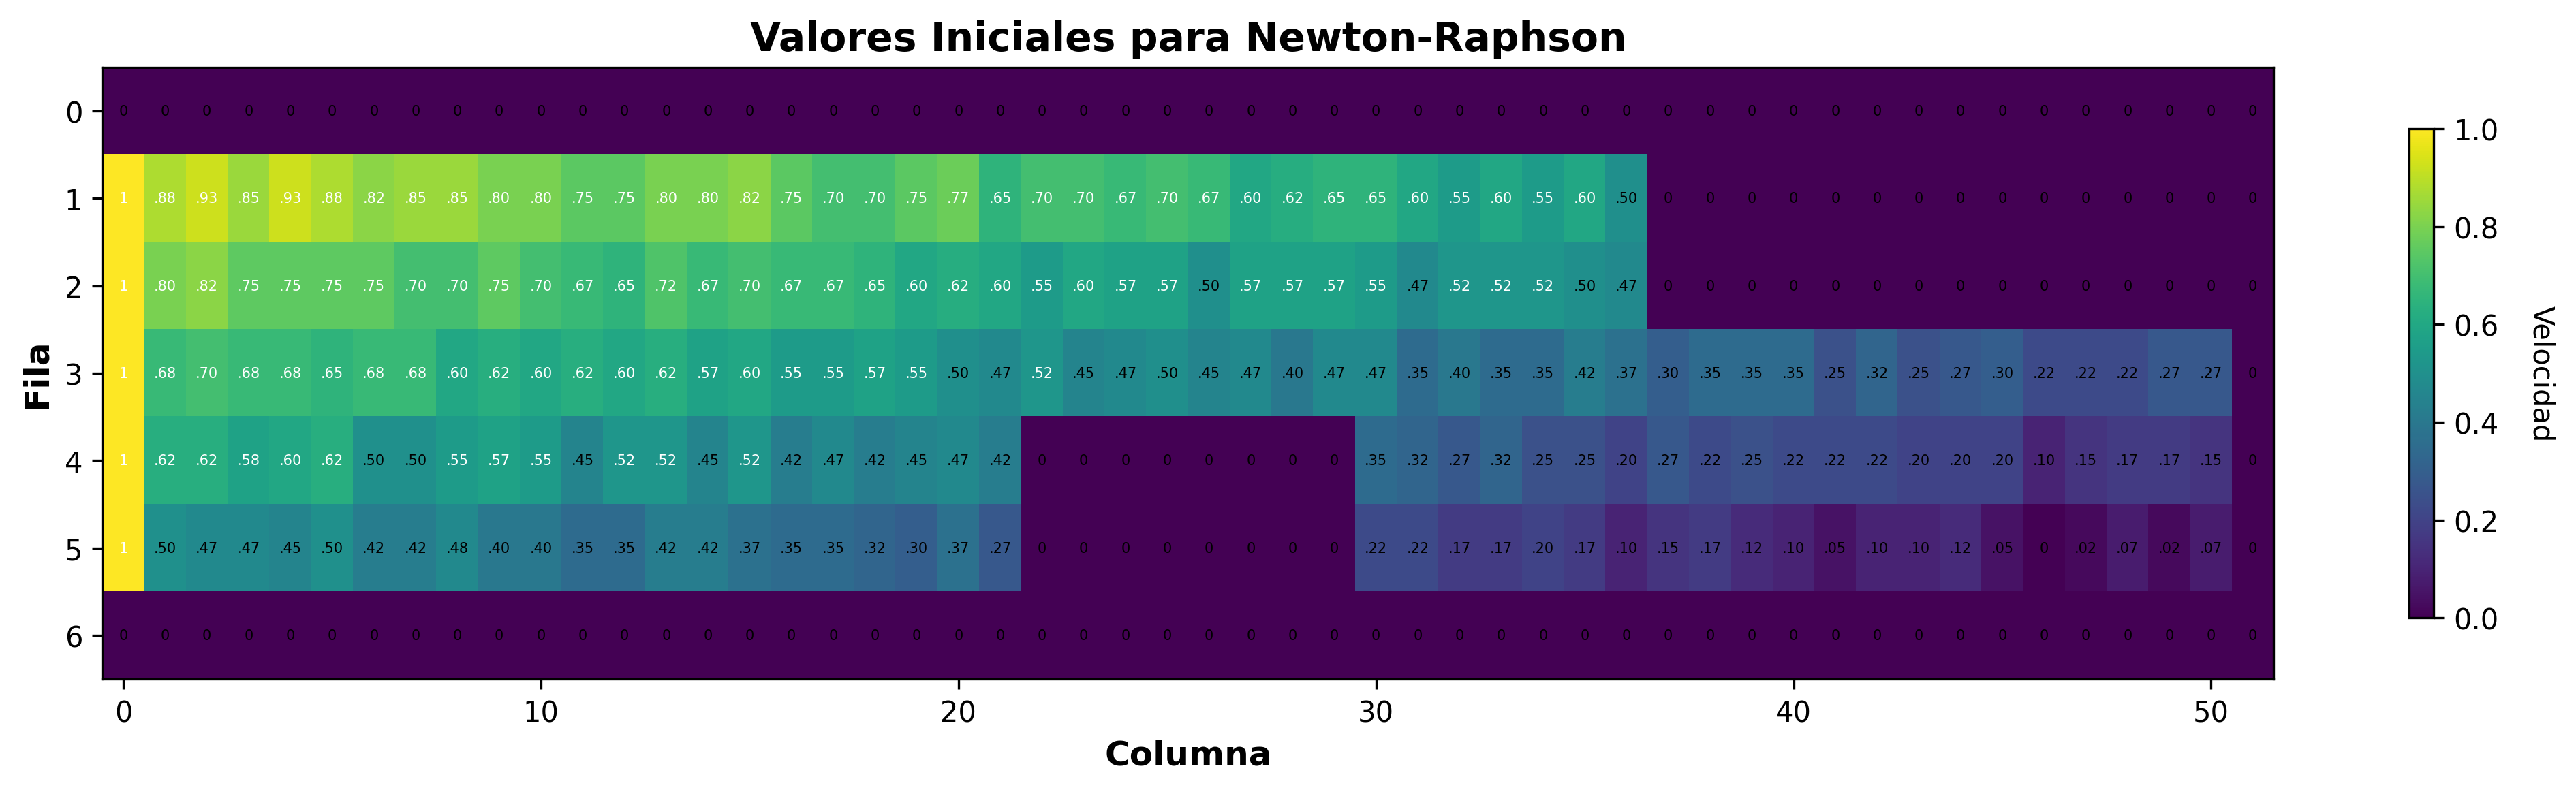
\includegraphics[width=0.9\textwidth]{seleccion_valores_iniciales.png}
\caption{Malla de valores iniciales generada con el algoritmo de selección informada. Los colores representan la magnitud de la velocidad.}
\label{fig:malla_inicial}
\end{figure}

Esta estrategia garantiza que:
\begin{itemize}
    \item Los valores disminuyen gradualmente de izquierda a derecha (simulando la pérdida de velocidad por fricción).
    \item Los valores disminuyen de arriba hacia abajo (reflejando el gradiente de velocidad típico).
    \item Hay variabilidad aleatoria dentro de cada región, evitando una inicialización demasiado uniforme.
\end{itemize}

\subsection{Cálculo del Vector de Residuales $\mathbf{F}(\mathbf{U})$}

El vector de residuales $\mathbf{F}(\mathbf{U})$ evalúa qué tan bien la solución actual satisface las ecuaciones discretizadas. Para cada nodo $(i,j)$ se calcula el residual correspondiente.

\subsubsection{Ecuación Discretizada Central}

Para nodos internos que no están en fronteras ni bloques, la ecuación de momento discretizada con diferencias finitas centradas es:

\[
v_{i,j}^2 = \frac{1}{4}\left( v_{i,j+1} + v_{i,j-1} + v_{i+1,j} + v_{i-1,j} - 4 v_{i,j}[v_{i,j+1} - v_{i,j-1}] - 4 V_y[v_{i-1,j} - v_{i+1,j}] \right)
\]

donde $V_y = -0.000005$ es la componente de velocidad en dirección $y$ (constante).

El residual para este nodo se define como:
\[
F_{i \times 52 + j} = -v_{i,j} + \frac{1}{4}\left( v_{i,j+1} + v_{i,j-1} + v_{i+1,j} + v_{i-1,j} - 4 v_{i,j}[v_{i,j+1} - v_{i,j-1}] - 4 V_y[v_{i-1,j} - v_{i+1,j}] \right)
\]

En forma vectorial, si $X_{\text{idx}} = v_{i,j}$ es el valor en el índice lineal $\text{idx} = i \times 52 + j$:

\[
\boxed{
F_{\text{idx}} = -X_{\text{idx}} + \frac{1}{4}\Big( X_{\text{idx}+1} + X_{\text{idx}-1} + X_{\text{idx}+52} + X_{\text{idx}-52} - 4 X_{\text{idx}}[X_{\text{idx}+1} - X_{\text{idx}-1}] - 4 V_y[X_{\text{idx}-52} - X_{\text{idx}+52}] \Big)
}
\]

\begin{figure}[H]
\centering
\includegraphics[width=0.95\textwidth]{ecuacion_residual.png}
\caption{Ecuación del residual $F_{i \cdot 52 + j}$ para cada punto de la malla. Esta ecuación representa el balance entre difusión y convección discretizado.}
\label{fig:ecuacion_residual}
\end{figure}

\subsubsection{Condiciones de Frontera}

Las condiciones de frontera se imponen directamente en el vector de residuales:

\paragraph{Frontera Izquierda (Inlet F):} $j = 0$
\begin{itemize}
    \item Para $i < i_{\text{bloque\_sup}}$: $v_{i,0} = v_0 = 1$
    \[
    F_{i \times 52 + 0} = v_{i,0} - 1 = 0 \quad \Rightarrow \quad F_{\text{idx}} = 0
    \]
    \item Para $i \geq i_{\text{bloque\_sup}}$: $v_{i,0} = 0$
    \[
    F_{i \times 52 + 0} = v_{i,0} = 0 \quad \Rightarrow \quad F_{\text{idx}} = 0
    \]
\end{itemize}

\paragraph{Frontera Superior (Surface G):} $i = 0$
\begin{itemize}
    \item Para $j < 37$: $v_{0,j} = v_0 = 1$
    \[
    F_{0 \times 52 + j} = v_{0,j} - 1 = 0 \quad \Rightarrow \quad F_{\text{idx}} = 0
    \]
    \item Para $j \geq 37$: $v_{0,j} = 0$
    \[
    F_{0 \times 52 + j} = v_{0,j} = 0 \quad \Rightarrow \quad F_{\text{idx}} = 0
    \]
\end{itemize}

\paragraph{Frontera Derecha (Outlet A):} $j = 51$
\[
v_{i,51} = 0 \quad \Rightarrow \quad F_{i \times 52 + 51} = 0
\]

\paragraph{Frontera Inferior (E):} $i = 6$
\[
v_{6,j} = 0 \quad \Rightarrow \quad F_{6 \times 52 + j} = 0
\]

\paragraph{Bloques Sólidos (B):}
Para cualquier nodo $(i,j)$ que esté dentro de un bloque:
\[
v_{i,j} = 0 \quad \Rightarrow \quad F_{i \times 52 + j} = 0
\]

Los bloques están definidos por:
\begin{itemize}
    \item \textbf{Bloque Superior:} $(37 \leq j \leq 50)$ y $(4 \leq i \leq 5)$
    \item \textbf{Bloque Inferior:} $(22 \leq j \leq 29)$ y $(1 \leq i \leq 2)$
\end{itemize}

\subsection{Cálculo de la Matriz Jacobiana $J(\mathbf{U})$}

La matriz Jacobiana es la derivada del vector de residuales respecto al vector de incógnitas:
\[
J_{pq} = \frac{\partial F_p}{\partial X_q}
\]

Es una matriz de dimensión $364 \times 364$ que es mayormente dispersa (sparse).

\subsubsection{Derivadas Parciales para Nodos Internos}

Para cualquier punto diferente a frontera, las derivadas parciales del residual son:

\begin{align}
\frac{\partial F_{i\cdot 52 + j}}{\partial X_{i\cdot 52 + j}} &= -1 - X_{i\cdot 52 + (j+1)} + X_{i\cdot 52 + (j-1)} \\[8pt]
\frac{\partial F_{i\cdot 52 + j}}{\partial X_{i\cdot 52 + (j+1)}} &= \tfrac{1}{4} - X_{i\cdot 52 + j} \\[8pt]
\frac{\partial F_{i\cdot 52 + j}}{\partial X_{i\cdot 52 + (j-1)}} &= \tfrac{1}{4} + X_{i\cdot 52 + j} \\[8pt]
\frac{\partial F_{i\cdot 52 + j}}{\partial X_{(i+1)\cdot 52 + j}} &= \tfrac{1}{4} - V_{y} \\[8pt]
\frac{\partial F_{i\cdot 52 + j}}{\partial X_{(i-1)\cdot 52 + j}} &= \tfrac{1}{4} + V_{y}
\end{align}

\subsubsection{Derivadas Parciales para Nodos de Frontera}

Para puntos en frontera o dentro de bloques:
\[
\frac{\partial F_{k}}{\partial X_{k}} = 1
\]

\subsubsection{Estructura de la Matriz Jacobiana}

La matriz Jacobiana tiene la siguiente estructura dispersa, donde las filas correspondientes a fronteras tienen 1 en la diagonal, y las filas interiores tienen 5 entradas no nulas:

\[
J \;=\;
\begin{pmatrix}
1 & 0 & 0 & 0 & \cdots & 0 & 0 & 0 \\
0 & 1 & 0 & 0 & \cdots & 0 & 0 & 0 \\
0 & 0 & 1 & 0 & \cdots & 0 & 0 & 0 \\
0 & 0 & 0 & 1 & \ddots & 0 & 0 & 0 \\
\vdots & \vdots & \vdots & \ddots & \ddots & \ddots & \vdots & \vdots \\[6pt]
\vdots & \vdots & \vdots & \cdots &
\frac{\partial F_{i\cdot 52 + j}}{\partial X_{i\cdot 52 + (j-1)}} &
\frac{\partial F_{i\cdot 52 + j}}{\partial X_{i\cdot 52 + j}} &
\frac{\partial F_{i\cdot 52 + j}}{\partial X_{i\cdot 52 + (j+1)}} &
\cdots \\[10pt]
\vdots & \vdots & \vdots & \cdots &
0 &
0 &
\cdots & \vdots \\[6pt]
0 & 0 & 0 & 0 & \cdots & 0 & 1 & 0 \\
0 & 0 & 0 & 0 & \cdots & 0 & 0 & 1 \\
\end{pmatrix}
\]

\begin{figure}[H]


\subsubsection{Mapa de calor del Jacobiano}

\includegraphics[width=1\textwidth]{jacobiano_heatmap.png}
\caption{Mapa de calor de la matriz Jacobiana ($364 \times 364$). Se observa la estructura dispersa con la diagonal dominante (azul/rojo) y las bandas secundarias correspondientes a los vecinos en la malla.}
\label{fig:jacobiana_heatmap}
\end{figure}

\subsection{Proceso Iterativo de Newton-Raphson}

El método de Newton-Raphson para sistemas no lineales se basa en la siguiente ecuación de iteración:
\[
\boxed{X_{i+1} = X_i + H}
\]

donde el incremento $H$ se obtiene resolviendo el sistema lineal $J \cdot H = -F(X)$. Calcular la inversa de la Jacobiana directamente es costoso y puede introducir errores numéricos; en su lugar, se utiliza un método iterativo para resolver el sistema lineal.

El algoritmo iterativo se describe a continuación:

\begin{algorithm}[H]
\caption{Método de Newton-Raphson para el Sistema No Lineal}
\begin{algorithmic}[1]
\STATE Inicializar $\mathbf{U}^{(0)}$ con la estrategia informada
\STATE Establecer tolerancias: $\varepsilon_F = 10^{-10}$, $\delta_{\text{step}} = 10^{-8}$
\STATE Establecer número máximo de iteraciones: $k_{\max} = 200$
\STATE $k \gets 0$
\STATE $\mathbf{U}_{\text{prev}} \gets \mathbf{U}^{(0)}$
\WHILE{$k < k_{\max}$}
    \STATE $k \gets k + 1$
    \STATE Calcular vector de residuales: $\mathbf{F}(\mathbf{U}^{(k-1)})$
    \STATE Calcular norma del residual: $\|\mathbf{F}\| = \|\mathbf{F}(\mathbf{U}^{(k-1)})\|_2$
    \STATE Imprimir: Iteración $k$, $\|\mathbf{F}\|$
    \IF{$\|\mathbf{F}\| < \varepsilon_F$}
        \STATE \textbf{Convergencia alcanzada} (Criterio 1: Norma del residual)
        \STATE \textbf{break}
    \ENDIF
    \STATE Calcular matriz Jacobiana: $J(\mathbf{U}^{(k-1)})$
    \STATE Resolver sistema lineal: $J(\mathbf{U}^{(k-1)}) \cdot \Delta\mathbf{U} = -\mathbf{F}(\mathbf{U}^{(k-1)})$
    \STATE Actualizar solución: $\mathbf{U}^{(k)} = \mathbf{U}^{(k-1)} + \Delta\mathbf{U}$
    \STATE Calcular cambio: $\varepsilon = \|\mathbf{U}^{(k)} - \mathbf{U}_{\text{prev}}\|_2$
    \STATE Imprimir: Epsilon (cambio) = $\varepsilon$
    \IF{$\varepsilon < \delta_{\text{step}}$}
        \STATE \textbf{Convergencia alcanzada} (Criterio 2: Cambio pequeño entre iteraciones)
        \STATE \textbf{break}
    \ENDIF
    \STATE $\mathbf{U}_{\text{prev}} \gets \mathbf{U}^{(k)}$
\ENDWHILE
\IF{$k = k_{\max}$}
    \STATE \textbf{No convergió} (Criterio 3: Número máximo de iteraciones alcanzado)
\ENDIF
\STATE \textbf{return} $\mathbf{U}^{(k)}$
\end{algorithmic}
\end{algorithm}

\subsection{Criterios de Parada}

La iteración se detiene cuando se cumple una de estas condiciones:

\begin{enumerate}
    \item \textbf{(C1) Norma del Residual:} La norma euclidiana del vector de residuales es suficientemente pequeña:
    \[
    \|\mathbf{F}(\mathbf{U}^{(k)})\|_2 = \sqrt{\sum_{i=1}^{364} F_i^2} < \varepsilon_F = 10^{-10}
    \]
    Este criterio verifica que todas las ecuaciones estén prácticamente satisfechas.
    
    \item \textbf{(C2) Epsilon (Cambio entre Iteraciones):} La solución deja de cambiar significativamente:
    \[
    \|\Delta\mathbf{U}^{(k)}\|_2 = \|\mathbf{U}^{(k)} - \mathbf{U}^{(k-1)}\|_2 < \delta_{\text{step}} = 10^{-8}
    \]
    Este criterio detecta cuando el método ha alcanzado un punto estacionario (aunque no necesariamente la solución exacta).
    
    \item \textbf{(C3) Límite de Iteraciones:} Se alcanza el número máximo de iteraciones:
    \[
    k \geq k_{\max} = 200
    \]
    Este criterio evita bucles infinitos en caso de no convergencia.
\end{enumerate}


\newpage
\section{Solución del Sistema Lineal: Elección del Método Iterativo}

En cada iteración del método de Newton-Raphson, debemos resolver el sistema lineal:
\[
J(\mathbf{U}^{(k)}) \cdot H = -\mathbf{F}(\mathbf{U}^{(k)})
\]

donde $H = \Delta\mathbf{U}^{(k)}$ es el incremento que buscamos. Este sistema tiene dimensión $364 \times 364$ (para nuestra malla de $52 \times 7$ nodos), lo que hace costoso el cálculo directo de la inversa. Por ello, analizamos diversos métodos iterativos para sistemas lineales.

\subsection{Marco Teórico: La Teoría de Separación (Splitting)}

El principio rector de los métodos iterativos estacionarios es convertir un problema difícil ($Ax = b$) en una secuencia de problemas fáciles \cite{Kincaid}. La idea es \textbf{separar la matriz A} en dos partes: una matriz $Q$ (fácil de invertir) y el resto $(Q - A)$.

\textbf{Derivación:} Partimos de $Ax = b$ y escribimos $A = Q - (Q - A)$:
\begin{align*}
Ax = b &\implies (Q - (Q-A))x = b \\
&\implies Qx - (Q-A)x = b
\end{align*}

Creamos una fórmula iterativa donde el lado izquierdo es el ``futuro'' $(k+1)$ y el derecho el ``presente'' $(k)$:
\[
Qx^{(k+1)} = (Q-A)x^{(k)} + b
\]

Multiplicando por $Q^{-1}$:
\begin{equation}
\boxed{x^{(k+1)} = (I - Q^{-1}A)x^{(k)} + Q^{-1}b = Gx^{(k)} + c}
\label{eq:splitting}
\end{equation}

donde $G = I - Q^{-1}A$ es la \textbf{matriz de iteración}. La elección de $Q$ determina el método.

\subsubsection{Teorema de Convergencia}

Un método iterativo de la forma (\ref{eq:splitting}) converge para cualquier punto inicial si y solo si:
\[
\boxed{\rho(G) < 1}
\]

donde $\rho(G) = \max|\lambda_i|$ es el \textbf{radio espectral} (el mayor valor absoluto de los valores propios de $G$).

\subsection{Métodos Analizados y Resultados}

Descomponemos la matriz $A$ en sus componentes: Diagonal ($D$), Triangular Inferior estricta ($-L$) y Triangular Superior estricta ($-U$), de modo que $A = D - L - U$.

\subsubsection{Método de Richardson}

Es la forma más simple de iteración. Elegimos $Q = I$ (la matriz identidad).

\textbf{Fórmula de actualización:}
\[
x^{(k+1)} = x^{(k)} + (b - Ax^{(k)}) = x^{(k)} + r^{(k)}
\]

donde $r^{(k)} = b - Ax^{(k)}$ es el \textbf{residuo}. La idea es: \emph{``Toma tu estimación actual y súmale el error que tienes''}.

\textbf{Resultado para nuestra Jacobiana:}
\[
\rho(G_{\text{Richardson}}) \approx 1.02 > 1 \quad \implies \quad \textbf{No converge}
\]

\subsubsection{Método de Jacobi}

Elegimos $Q = D$ (la diagonal de $A$), que es trivial de invertir: $(D^{-1})_{ii} = 1/a_{ii}$.

\textbf{Fórmula de actualización:}
\[
x^{(k+1)} = D^{-1}(L + U)x^{(k)} + D^{-1}b
\]

Por componentes, cada variable $x_i$ se calcula usando solo valores del paso anterior:
\[
x_i^{(k+1)} = \frac{1}{a_{ii}} \left( b_i - \sum_{j \neq i} a_{ij} x_j^{(k)} \right)
\]

\textbf{Requisito:} Converge garantizadamente si $A$ es \textbf{diagonalmente dominante estricta}:
\[
|a_{ii}| > \sum_{j \neq i} |a_{ij}|, \quad \forall i
\]

\textbf{Resultado para nuestra Jacobiana:}
\begin{itemize}
    \item La Jacobiana \textbf{NO} es diagonalmente dominante
    \item $\rho(G_{\text{Jacobi}}) \approx 1.49 > 1 \quad \implies \quad \textbf{No converge}$
\end{itemize}

\subsubsection{Método de Gauss-Seidel}

Mejora de Jacobi: si ya calculamos $x_1^{(k+1)}$, ¿por qué usar el viejo $x_1^{(k)}$ para calcular $x_2^{(k+1)}$?

Elegimos $Q = D - L$ (diagonal + triángulo inferior).

\textbf{Fórmula de actualización:}
\[
x^{(k+1)} = (D - L)^{-1} U x^{(k)} + (D - L)^{-1} b
\]

\textbf{Requisito:} También requiere dominancia diagonal o que $A$ sea simétrica definida positiva.

\textbf{Resultado para nuestra Jacobiana:}
\[
\rho(G_{\text{Gauss-Seidel}}) \approx 2.22 > 1 \quad \implies \quad \textbf{No converge}
\]

\subsubsection{Método de Gradiente Descendente}

Este método cambia el paradigma: en lugar de álgebra lineal, usa \textbf{cálculo}. Si la matriz $A$ es Simétrica y Definida Positiva (SDP), resolver $Ax = b$ equivale a minimizar la función cuadrática:
\[
f(x) = \frac{1}{2}x^T A x - b^T x, \qquad \nabla f(x) = Ax - b
\]

\textbf{Demostración:} El mínimo ocurre cuando $\nabla f(x) = Ax - b = 0$, es decir, $Ax = b$.

\textbf{Algoritmo:} Desde un punto $x^{(k)}$, caminamos en la dirección de máximo descenso (el negativo del gradiente, que es el residuo $r^{(k)} = b - Ax^{(k)}$):
\[
x^{(k+1)} = x^{(k)} + \alpha_k r^{(k)}
\]

donde el paso óptimo $\alpha_k$ se calcula minimizando $f(x^{(k)} + \alpha r^{(k)})$:
\[
\alpha_k = \frac{r^{(k)T} r^{(k)}}{r^{(k)T} A r^{(k)}}
\]

\textbf{Requisito:} La matriz $A$ debe ser \textbf{simétrica} ($A^T = A$) y \textbf{definida positiva} ($x^T A x > 0, \forall x \neq 0$).

\textbf{Problema:} Nuestra Jacobiana $J$ \textbf{NO} es simétrica ($J^T \neq J$), por lo que no se puede aplicar directamente.

\textbf{Resultado (si se forzara):}
\[
\rho(G_{\text{Grad.Desc.}}) \approx 0.99992 < 1 \quad \implies \quad \text{Converge, pero \textbf{muy lentamente}}
\]

\subsection{Resumen de Métodos Analizados}

La siguiente tabla resume las fórmulas de actualización de cada método y su idea clave:

\begin{table}[H]
\centering
\begin{tabular}{|l|l|l|}
\hline
\textbf{Método} & \textbf{Fórmula} & \textbf{Idea Clave} \\
\hline
Richardson & $x + (b - Ax)$ & Usa el error directamente \\
Jacobi & $D^{-1}(L+U)x + D^{-1}b$ & Actualiza con datos viejos \\
Gauss-Seidel & $(D-L)^{-1}Ux + (D-L)^{-1}b$ & Usa datos nuevos al instante \\
Grad. Descendente & $x + \alpha r$ & Baja por pendiente máxima \\
Grad. Conjugado & $x + \alpha d$ (conjugado) & Pendiente ``inteligente'' \\
\hline
\end{tabular}
\caption{Resumen de fórmulas de actualización de métodos iterativos.}
\end{table}

La siguiente tabla muestra los resultados de convergencia para nuestra matriz Jacobiana:

\begin{table}[H]
\centering
\begin{tabular}{|l|c|c|l|}
\hline
\textbf{Método} & \textbf{Radio Espectral $\rho(G)$} & \textbf{¿Converge?} & \textbf{Razón del fallo} \\
\hline
Richardson & $\approx 1.02$ & No & $\rho > 1$ \\
Jacobi & $\approx 1.49$ & No & No hay dominancia diagonal \\
Gauss-Seidel & $\approx 2.22$ & No & No hay dominancia diagonal \\
Grad. Descendente & $\approx 0.99992$ & Muy lento & $J$ no es simétrica \\
\hline
\end{tabular}
\caption{Comparación de métodos iterativos para la matriz Jacobiana.}
\label{tab:metodos}
\end{table}

\subsection{El Problema con la Matriz Jacobiana}

Nuestra matriz Jacobiana $J \in \mathbb{R}^{364 \times 364}$ presenta las siguientes características:

\begin{itemize}
    \item \textbf{No es simétrica:} $J^T \neq J$
    \item \textbf{No es definida positiva:} Tiene valores propios negativos (algunos: $-3.38, -3.26, -3.14, \ldots$)
    \item \textbf{No es diagonalmente dominante}
    \item \textbf{Número de condición:} $\kappa(J) \approx 24.02$
\end{itemize}

Estas propiedades hacen que los métodos iterativos clásicos \textbf{no converjan} o converjan demasiado lento. La solución es multiplicar por $J^T$ para obtener $J^T J$ que sí es simétrica y definida positiva, permitiendo usar Gradiente Conjugado.

\subsection{La Solución: Transformación a Sistema Simétrico Definido Positivo}

Para aplicar el método de Gradiente Conjugado (que requiere matriz SDP), transformamos el sistema original multiplicando ambos lados por $J^T$:

\textbf{Sistema original:}
\[
J \cdot H = -F(X)
\]

\textbf{Sistema transformado:}
\[
\boxed{J^T J \cdot H = -J^T F(X)}
\]

\subsubsection{Propiedades de $A = J^T J$}

\begin{enumerate}
    \item \textbf{Simétrica:} $(J^T J)^T = J^T (J^T)^T = J^T J$ \checkmark
    \item \textbf{Definida Positiva:} Para cualquier $x \neq 0$:
    \[
    x^T (J^T J) x = (Jx)^T (Jx) = \|Jx\|^2 \geq 0
    \]
    y es estrictamente positivo si $J$ tiene rango completo (todas las ecuaciones son independientes).
    \item \textbf{Invertible:} Si $\text{rank}(J) = n$, entonces $J^T J$ es invertible.
\end{enumerate}

\subsubsection{Efecto en el Número de Condición}

El \textbf{número de condición} $\kappa(A) = \|A\|_2 \cdot \|A^{-1}\|_2$ mide la sensibilidad del sistema a errores numéricos \cite{Golub}:

\begin{itemize}
    \item Número de condición de $J$: $\kappa(J) \approx 24.02$
    \item Número de condición de $J^T J$: $\kappa(J^T J) \approx 577.08 - 689.39$
\end{itemize}

\textbf{Observación:} El número de condición aumenta al cuadrado ($\kappa(J^T J) \approx \kappa(J)^2$), lo que hace el sistema más sensible a errores numéricos. Sin embargo, ahora \textbf{sí podemos} aplicar Gradiente Conjugado, que tiene convergencia garantizada.

\subsection{Método de Gradiente Conjugado}

El Gradiente Conjugado es el ``santo grial'' de los métodos iterativos para matrices SDP \cite{Shewchuk}. En lugar de seguir la dirección del gradiente (que causa zigzag), busca direcciones \textbf{$A$-conjugadas} (ortogonales respecto a la matriz $A$). La matriz $A$ debe cumplir: $A \in \mathbb{R}^{n \times n}$, $A^T = A$, y $\mathbf{x}^T A \mathbf{x} > 0$ para todo $\mathbf{x} \neq 0$.

\subsubsection{Definición de Direcciones Conjugadas}

Dos vectores $d_i$ y $d_j$ son \textbf{conjugados} respecto a $A$ si:
\[
d_i^T A d_j = 0, \quad i \neq j
\]

Esto significa que moverse en la dirección $d_j$ no ``arruina'' la minimización que ya hicimos en $d_i$.

\subsubsection{Algoritmo de Gradiente Conjugado}

\begin{algorithm}[H]
\caption{Gradiente Conjugado para $AH = b$}
\begin{algorithmic}[1]
\STATE $H^{(0)} = 0$ (estimación inicial)
\STATE $r^{(0)} = b - A H^{(0)} = b$ (residuo inicial)
\STATE $d^{(0)} = r^{(0)}$ (dirección inicial = gradiente)
\FOR{$k = 0, 1, 2, \ldots$ hasta convergencia}
    \STATE $\alpha_k = \frac{r^{(k)T} r^{(k)}}{d^{(k)T} A d^{(k)}}$ \COMMENT{Tamaño del paso}
    \STATE $H^{(k+1)} = H^{(k)} + \alpha_k d^{(k)}$ \COMMENT{Actualizar solución}
    \STATE $r^{(k+1)} = r^{(k)} - \alpha_k A d^{(k)}$ \COMMENT{Actualizar residuo}
    \IF{$\|r^{(k+1)}\| < \varepsilon \|r^{(0)}\|$}
        \STATE \textbf{Convergencia alcanzada}
        \STATE \textbf{break}
    \ENDIF
    \STATE $\beta_k = \frac{r^{(k+1)T} r^{(k+1)}}{r^{(k)T} r^{(k)}}$ \COMMENT{Coeficiente de conjugación}
    \STATE $d^{(k+1)} = r^{(k+1)} + \beta_k d^{(k)}$ \COMMENT{Nueva dirección conjugada}
\ENDFOR
\end{algorithmic}
\end{algorithm}

\subsubsection{Ventajas del Gradiente Conjugado}

\begin{itemize}
    \item \textbf{Convergencia garantizada:} Para una matriz SDP de tamaño $n$, converge en máximo $n$ iteraciones (teóricamente exacto).
    \item \textbf{Sin zigzag:} Las direcciones conjugadas evitan repetir trabajo.
    \item \textbf{Bajo costo por iteración:} Solo requiere multiplicaciones matriz-vector.
\end{itemize}

\subsection{Criterios de Parada del Gradiente Conjugado}

En nuestra implementación, el Gradiente Conjugado interno se detiene cuando:

\begin{enumerate}
    \item \textbf{Norma del residuo relativa:}
    \[
    \|r^{(k)}\|_2 < \varepsilon \cdot \|r^{(0)}\|_2, \quad \varepsilon = 10^{-10}
    \]
    
    \item \textbf{Límite de iteraciones:} $k \geq 364$ (dimensión del sistema)
    
    \item \textbf{Evitación de división por cero:} Si $|d^{(k)T} A d^{(k)}| < 10^{-30}$, indica que la matriz está mal condicionada.
\end{enumerate}

\subsection{Resultados de la Implementación}

Con la transformación $J^T J$ y el método de Gradiente Conjugado, obtuvimos los siguientes resultados:

\begin{table}[H]
\centering
\begin{tabular}{|l|c|}
\hline
\textbf{Métrica} & \textbf{Valor} \\
\hline
Iteraciones promedio de Gradiente Conjugado (por paso Newton) & $\sim 100$ \\
Iteraciones promedio de Newton-Raphson hasta convergencia & $\sim 116$ \\
Número de condición de $J$ & $24.02 - 1184.53$ \\
Número de condición de $J^T J$ & $577.08 - 689.39$ \\
Criterio de convergencia alcanzado & Epsilon $< 10^{-8}$ \\
Valor máximo final en la malla & $1.0000$ \\
Valor mínimo final en la malla & $\sim 0$ \\
\hline
\end{tabular}
\caption{Resultados de convergencia del método implementado.}
\end{table}

\subsection{Implementación y Resultados}

El método fue implementado en Python usando las bibliotecas NumPy para álgebra lineal y Matplotlib para visualización. El código incluye:

\begin{itemize}
    \item Clase \texttt{Malla}: Gestiona la geometría, condiciones de frontera y valores iniciales
    \item Clase \texttt{Bloque}: Define los obstáculos sólidos
    \item Clase \texttt{Vector}: Implementa el cálculo de $\mathbf{F}(\mathbf{U})$, $J(\mathbf{U})$, la transformación $J^T J$ y el método de Gradiente Conjugado para resolver el sistema lineal en cada iteración
    \item Función principal que ejecuta el ciclo de Newton-Raphson con monitoreo en tiempo real del número de condición, valores propios y convergencia del Gradiente Conjugado interno
\end{itemize}

El sistema lineal $J \cdot H = -F(X)$ se resuelve mediante la transformación $J^T J \cdot H = -J^T F(X)$, que permite aplicar el método de Gradiente Conjugado gracias a que $J^T J$ es simétrica y definida positiva.

\subsubsection{Mapa de calor con valores numéricos}

% ESPACIO PARA FIGURA DE RESULTADOS
\begin{figure}[H]
\centering
\includegraphics[width=0.9\textwidth]{malla_final.png}
\caption{Malla de valores finales después de la convergencia del método de Newton-Raphson. Se observa la distribución de velocidades resultante.}
\label{fig:malla_final}
\end{figure}


\subsubsection{Mapa de calor}
\begin{figure}[H]

\includegraphics[width=0.9\textwidth]{malla_final_2.png}
\caption{Malla de valores finales después de la convergencia del método de Newton-Raphson. Se observa la distribución de velocidades resultante.}
\label{fig:malla_final}
\end{figure}



\subsection{Refinamiento Visual mediante Interpolación}

Para mejorar la calidad de visualización en la malla reducida ($50\times5$), se aplicó interpolación mediante splines cúbicos bidimensionales \cite{SciPy}. Esta técnica permite generar representaciones suavizadas del campo de velocidades sin modificar los valores calculados originalmente.

\subsubsection{Metodología de Interpolación}

Se utiliza la función \texttt{RectBivariateSpline} de SciPy con los siguientes parámetros:
\begin{itemize}
    \item \textbf{Orden de los splines:} $k_x = k_y = 3$ (cúbicos)
    \item \textbf{Factor de suavizado:} $s = 0$ (interpolación exacta en los nodos)
    \item \textbf{Factor de refinamiento:} $f = 10$ (genera $10\times$ más puntos por eje)
\end{itemize}

Esto resulta en una malla de visualización de $(50-1)\times10 + 1 = 491$ puntos en dirección $x$ y $(5-1)\times10 + 1 = 41$ puntos en dirección $y$, proporcionando una representación visual continua del campo de velocidades.

\subsubsection{Visualización de la Función de Interpolación}

Para comprender mejor la naturaleza de la interpolación spline, se generan dos visualizaciones complementarias que muestran el comportamiento de la función escalar $S(x,y)$ construida a partir de los valores nodales:

\paragraph{Superficie 3D del Spline.} La función de interpolación $S: [0, 49] \times [0, 4] \to \mathbb{R}$ se puede visualizar como una superficie tridimensional donde:
\begin{itemize}
    \item Los ejes horizontales ($x$, $y$) representan las coordenadas de la malla
    \item El eje vertical representa el valor de velocidad $u(x,y)$
    \item La superficie es $C^2$-continua (derivadas segundas continuas) gracias al orden cúbico del spline
\end{itemize}

\begin{figure}[H]
\centering

\includegraphics[width=0.95\textwidth]{spline_superficie_3d.png}
\caption{Superficie 3D de la función de interpolación spline cúbico bidimensional. Se observa claramente la variación del campo de velocidades: valores altos en la entrada (izquierda superior) que decrecen gradualmente hacia la salida (derecha inferior), con valles correspondientes a las zonas de los bloques.}
\label{fig:spline_3d}
\end{figure}

\paragraph{Cortes y Perfiles de Velocidad.} Para analizar el comportamiento del spline en detalle, se trazan cortes de la función a lo largo de líneas de $y$ constante (perfiles horizontales) y $x$ constante (perfiles verticales):

\begin{figure}[H]
\centering

\includegraphics[width=0.95\textwidth]{spline_cortes.png}
\caption{Análisis de la función de interpolación mediante cortes. \textbf{Superior izquierda:} Perfiles horizontales mostrando la variación de velocidad a diferentes alturas. \textbf{Superior derecha:} Perfiles verticales mostrando la distribución en diferentes secciones del canal. \textbf{Inferior izquierda:} Curvas de nivel (contornos) de la superficie. \textbf{Inferior derecha:} Mapa de calor con isolíneas superpuestas.}
\label{fig:spline_cortes}
\end{figure}

Los perfiles permiten identificar:
\begin{itemize}
    \item La suavidad de la interpolación sin oscilaciones espurias
    \item La monotonía de los perfiles en regiones alejadas de los obstáculos
    \item Las perturbaciones localizadas causadas por la presencia de los bloques
\end{itemize}

\subsubsection{Resultado Final Suavizado}

Aplicando la interpolación a toda la malla, se obtiene el campo de velocidades refinado:

\begin{figure}[H]
\centering

\includegraphics[width=0.95\textwidth]{malla_suavizada.png}
\caption{Campo de velocidades suavizado mediante interpolación con splines cúbicos. La visualización refinada muestra claramente la distribución de velocidades desde la entrada (izquierda, valores altos en amarillo) hasta la salida (derecha, valores bajos en azul), con las zonas de los bloques en velocidad cero.}
\label{fig:malla_suavizada}
\end{figure}

\subsection{Observaciones sobre la Convergencia}

Durante la ejecución del algoritmo se observa:

\begin{itemize}
    \item La norma del residual $\|\mathbf{F}\|$ disminuye rápidamente en las primeras iteraciones (convergencia cuadrática característica de Newton-Raphson).
    \item El Gradiente Conjugado interno típicamente converge en $\sim 100$ iteraciones, aunque ocasionalmente detecta matrices mal condicionadas.
    \item La inicialización informada (valores decrecientes de izquierda a derecha y de arriba a abajo) mejora significativamente la convergencia.
    \item La transformación $J^T J$ permite usar Gradiente Conjugado a costa de aumentar el número de condición.
\end{itemize}

\newpage
\section{Conclusiones y Próximos Pasos}

\textbf{Conclusiones.} Se ha establecido un marco teórico y numérico sólido para la simulación. Se formalizó la geometría, las mallas, la discretización por diferencias finitas y el catálogo completo de las ecuaciones especiales para el tratamiento de fronteras. Crucialmente, se ha definido e implementado:

\begin{itemize}
    \item Una estrategia de inicialización informada para el método de Newton-Raphson, adaptada a la física esperada del problema.
    \item El cálculo completo del vector de residuales $\mathbf{F}(\mathbf{U})$ incluyendo todas las condiciones de frontera.
    \item El cálculo de la matriz Jacobiana $J(\mathbf{U})$ con derivadas parciales exactas.
    \item Tres criterios de parada robustos para garantizar la convergencia o detectar problemas.
    \item Implementación funcional en Python con visualización de resultados.
\end{itemize}

\textbf{Próximos Pasos.}
\begin{itemize}[leftmargin=1.25em]
    \item \textbf{Validación Extendida:} Verificar la convergencia y estabilidad del método en diferentes condiciones iniciales y parámetros físicos.
    
    \item \textbf{Optimización para Mallas Grandes:} Implementar técnicas de matrices dispersas (sparse matrices) para reducir el costo computacional al escalar a $h=1$.
    
    \item \textbf{Integración del Sistema Completo:} Levantar las simplificaciones actuales. Esto implica:
    \begin{itemize}
        \item Discretizar e incorporar la ecuación de momento para la componente $v_y$.
        \item Implementar un método para satisfacer la ecuación de continuidad (ej., un esquema de corrección de presión o la formulación de vorticidad-función de corriente).
    \end{itemize}
    
    \item \textbf{Análisis y Escalado:} Una vez validado el modelo completo, ejecutar la simulación en la malla fina ($400 \times 40$ con $h=1$) y analizar los resultados.
    
    \item \textbf{Visualización Avanzada:} Generar gráficos de campos vectoriales, líneas de corriente y contornos de vorticidad para interpretar físicamente la interacción del flujo con los obstáculos.
    
    \item \textbf{Análisis de Sensibilidad:} Estudiar cómo varían los resultados con diferentes valores de $V_y$, diferentes geometrías de bloques y diferentes condiciones de frontera.
\end{itemize}

\begin{thebibliography}{9}
\bibitem{LandauPaez}
R.~Landau \& M.~Páez.
\newblock \emph{Computational Problems for Physics: With Guided Solutions Using Python}.
\newblock CRC Press, 2018. Cap.~4.6 Hidrodinámica (Navier–Stokes, viga sumergida, vorticidad).

\bibitem{NumRec}
W.~Press, S.~Teukolsky, W.~Vetterling \& B.~Flannery.
\newblock \emph{Numerical Recipes: The Art of Scientific Computing}.
\newblock Cambridge University Press, 3rd Edition, 2007.

\bibitem{Burden}
R.~Burden \& J.~Faires.
\newblock \emph{Análisis Numérico}.
\newblock Cengage Learning, 9th Edition, 2011.

\bibitem{Kincaid}
D.~Kincaid \& W.~Cheney.
\newblock \emph{Numerical Analysis: Mathematics of Scientific Computing}.
\newblock Brooks/Cole, 3rd Edition, 2002.

\bibitem{Shewchuk}
J.~R.~Shewchuk.
\newblock \emph{An Introduction to the Conjugate Gradient Method Without the Agonizing Pain}.
\newblock Carnegie Mellon University, 1994.

\bibitem{SciPy}
P.~Virtanen et al.
\newblock \emph{SciPy 1.0: Fundamental Algorithms for Scientific Computing in Python}.
\newblock Nature Methods, 17:261–272, 2020.

\bibitem{Golub}
G.~H.~Golub \& C.~F.~Van Loan.
\newblock \emph{Matrix Computations}.
\newblock Johns Hopkins University Press, 4th Edition, 2013.
\end{thebibliography}

\end{document}